\documentclass[12pt]{article}


\usepackage{graphicx}
\usepackage{caption}
\usepackage{float}
\usepackage{subcaption}

\usepackage{amsmath}
\usepackage{algorithm}
\usepackage[noend]{algpseudocode}

\makeatletter
\def\BState{\State\hskip-\ALG@thistlm}
\makeatother

\usepackage[hidelinks]{hyperref}


\usepackage[nameinlink]{cleveref}
\AtBeginDocument{%
  \crefname{equation}{برابری}{equations}%
  \crefname{chapter}{فصل}{chapters}%
  \crefname{section}{بخش}{sections}%
  \crefname{appendix}{پیوست}{appendices}%
  \crefname{enumi}{مورد}{items}%
  \crefname{footnote}{زیرنویس}{footnotes}%
  \crefname{figure}{شکل}{figures}%
  \crefname{table}{جدول}{tables}%
  \crefname{theorem}{قضیه}{theorems}%
  \crefname{lemma}{لم}{lemmas}%
  \crefname{corollary}{نتیجه}{corollaries}%
  \crefname{proposition}{گزاره}{propositions}%
  \crefname{definition}{تعریف}{definitions}%
  \crefname{result}{نتیجه}{results}%
  \crefname{example}{مثال}{examples}%
  \crefname{remark}{نکته}{remarks}%
  \crefname{note}{یادداشت}{notes}%
  \crefname{observation}{مشاهده}{observations}%
  \crefname{algorithm}{الگوریتم}{algorithms}%
  \crefname{cproof}{برهان}{cproofs}%
}

\usepackage{xepersian}

\settextfont{XB Zar}[
  Path=./fonts/,
  Scale=1.2,
  Extension=.TTF,
  UprightFont=*,
  ItalicFont=*It,
  BoldFont=*Bd,
  BoldItalicFont=*BdIt
]

\setdigitfont{XB Zar}[
  Path=./fonts/,
  Scale=1.2,
  Extension=.TTF,
  UprightFont=*,
  ItalicFont=*It,
  BoldFont=*Bd,
  BoldItalicFont=*BdIt
]

\setlatintextfont[Scale=1.1]{Times New Roman}

% \setmonofont[
%   Path=./fonts/,
%   Scale=1.0,
%   Weight=800,
%   Extension=.TTF,
% ]{Inconsolata}


\title{مقایسهٔ الگوریتم‌های مرتب‌سازی}
\author{محمد ترابی - علی جعفر‌آبادی - رضا تاج‌گذاری} 
\date{تیرماه ۱۴۰۲}

\newtheorem{remark}{نکته}
\newtheorem{example}{مثال}

\begin{document}
\maketitle

\pagebreak

\section{مرتب‌سازی درجی\protect\LTRfootnote{Insertion sort}}

اگر یک دسته کارت به شما داده شود که اعداد ۱ تا ۵۰ روی آن نوشته شده است، چگونه آن را مرتب\LTRfootnote{sort}
می‌کنید؟
احتمالا اول تعداد کمی کارت برمی‌دارید و آن‌ها را مرتب می‌کنید؛
سپس بقیه کارت‌ها را یکی پس از دیگری نگاه می‌کنید
و در جای مناسب میان کارت‌های مرتب شده قرار می‌دهید.
\cref{fig:f1}
نمایی کلی از این روش مرتب‌سازی نشان می‌دهد.

وقتی کارت‌ها را با این روند مرتب می‌کنیم،
همواره تعدادی از کارت‌ها مرتب شده است و کارت‌هایی که هنوز مرتب نشده، یکی پس از دیگری
در دستهٔ کارت‌های مرتب شده درج\LTRfootnote{insert}
می‌شوند.
اگر با این روش کارت‌ها را مرتب کنیم، درواقع از مرتب‌سازی درجی استفاده کرده‌ایم.

\begin{figure}[H]
  \centering
  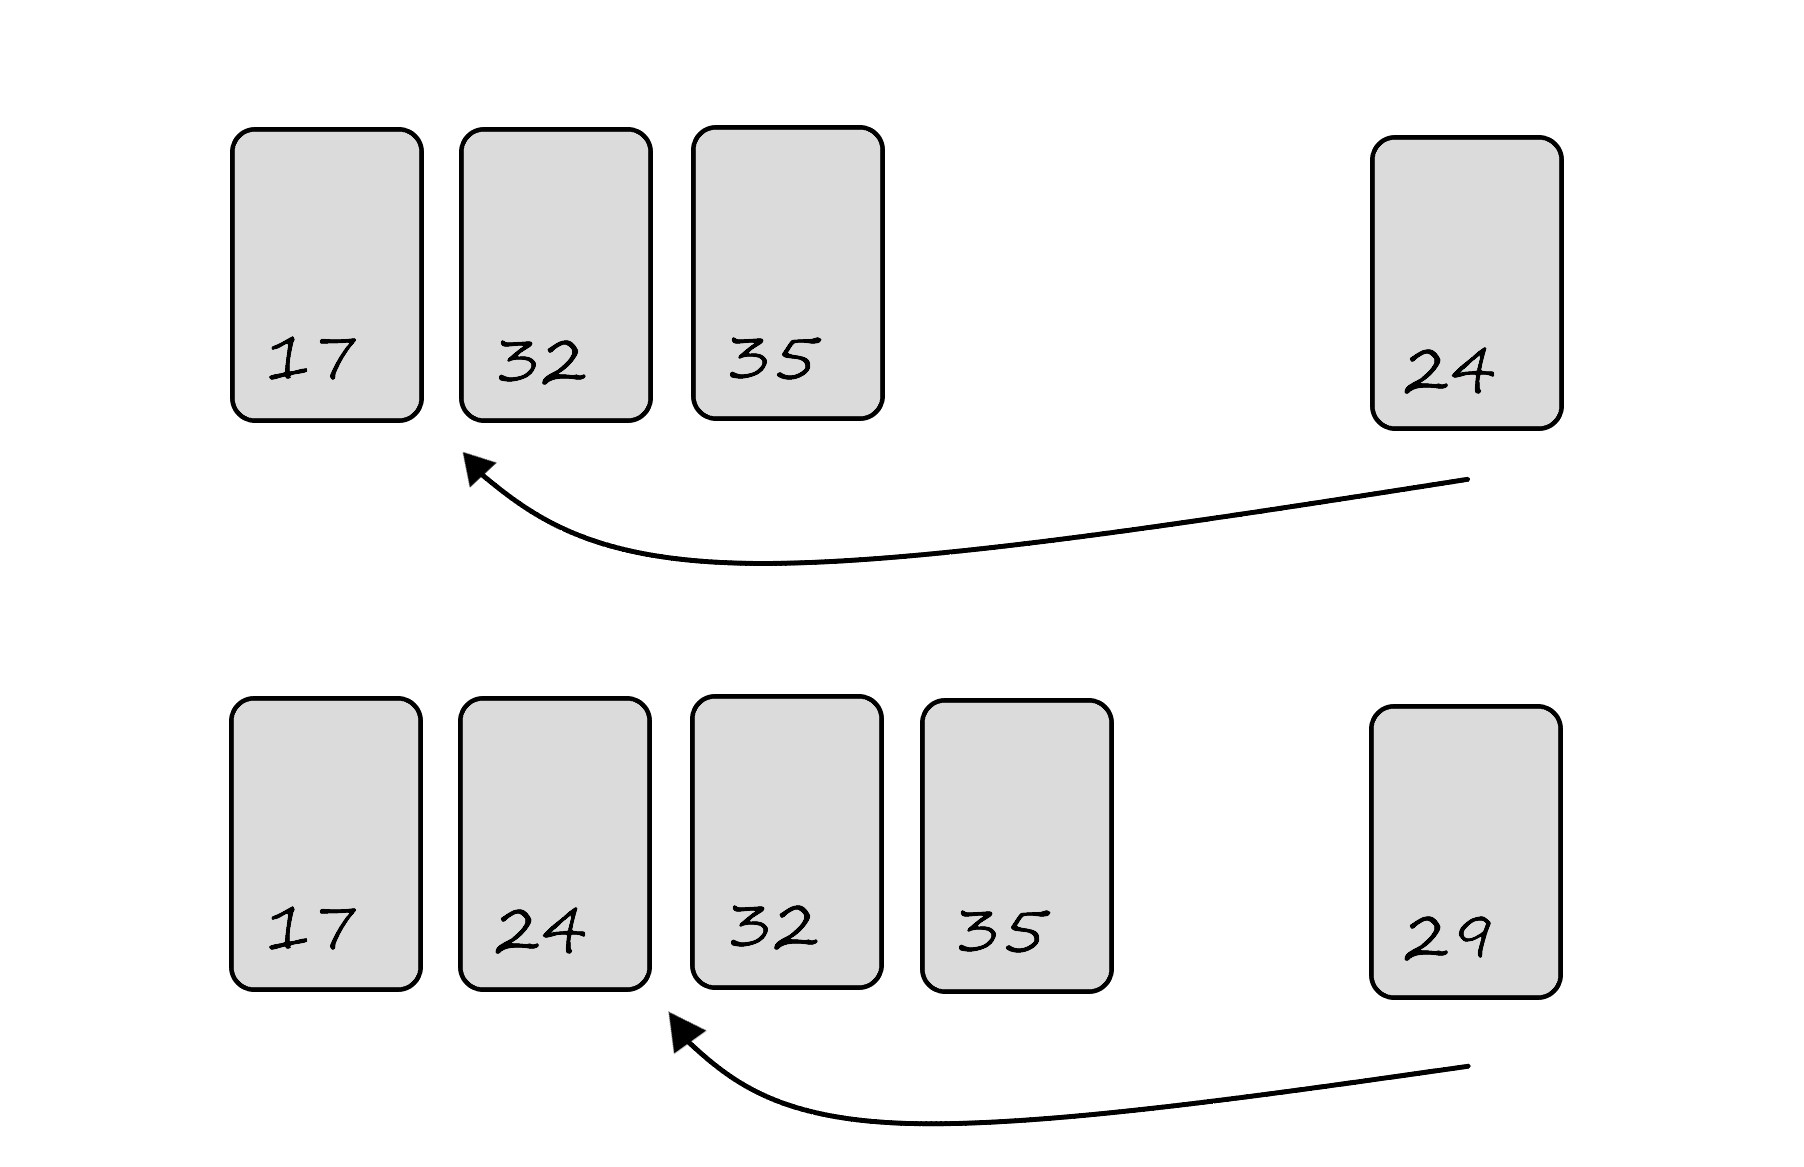
\includegraphics[width=.8\textwidth]{figs/sortingCards2.jpg}
  \caption{
    مراحلی از مرتب کردن کارت‌ها به کمک مرتب‌سازی درجی
  }
  \label{fig:f1}
\end{figure}

\subsection*{الگوریتم مرتب‌سازی درجی}
آرایه‌ای به طول یک همواره مرتب است؛ بنابراین از عنصر دوم شروع می‌کنیم و جلو می‌رویم.
فرض کنیم که به عنصر
$i$
رسیده‌ایم،
عناصر قبل از
$i$
مرتب‌اند.
لذا از آخرین عنصر قبل از
$i$
شروع می‌کنیم و به عقب می‌رویم.
هر یک از عناصر بزرگتر از
$i$
را یک واحد به سمت راست انتقال\LTRfootnote{shift}
می‌دهیم.
وقتی به عنصری کوچک تر از
$i$
یا به ابتدای آرایه رسیدیم
متوقف می‌شویم و
$i$
را همانجا درج
می‌کنیم.
هنگامی که عنصر
$i$
را درج می‌کنیم،
$i$
عنصر اول آرایه مرتب می‌شوند.
بنابراین این کار را ادامه می‌دهیم تا تمام عناصر آرایه مرتب شوند.
درستی مرتب‌سازی درجی را می‌توان به کمک ثابت‌های حلقه\LTRfootnote{loop invariants}
اثبات کرد.
\cite{clrs}
شبه‌کد مرتب‌سازی درجی را می‌توانید در
\cref{alg:a1}
که در ادامه آمده است
مشاهده کنید
\footnote{
  توجه داشته باشید که الگوریتم بر پایه صفر است؛ یعنی عنصر اول آرایه
  $arr[0]$
  می‌باشد.
}
.

\begin{algorithm}[H]
  \caption{مرتب‌سازی درجی}
  \label{alg:a1}
  \begin{latin}
    \begin{algorithmic}[1]
      \Procedure{InsertionSort}{arr, n}
      \For {$i \gets 1$ \textbf{to} $n-1$}
      \State $key \gets arr[i]$
      \State $j \gets i-1$
      \While {$j >= 0$ and $arr[j] > key$}
      \State $arr[j+1] \gets arr[j]$
      \State $j \gets j - 1$
      \EndWhile
      \State $arr[j+1] \gets key$
      \EndFor
      \EndProcedure
    \end{algorithmic}
  \end{latin}
\end{algorithm}

\begin{example}
  اگر الگوریتم بالا را روی آرایهٔ
  $[7, 6, 6, 4, 9]$
  اجرا کنیم،
  آرایه بدین صورت مرتب می‌شود:
  \begin{align*}
     & [7, 6, 6, 4, 9] \rightarrow [7, 7, 6, 4, 9] \rightarrow
    [6, 7, 6, 4, 9] \rightarrow [6, 7, 7, 4, 9] \rightarrow    \\
     & [6, 6, 7, 4, 9] \rightarrow [6, 6, 7, 7, 9] \rightarrow
    [6, 6, 6, 7, 9] \rightarrow [6, 6, 6, 7, 9]  \rightarrow   \\
     & [4, 6, 6, 7, 9] \rightarrow [4, 6, 6, 7, 9]
  \end{align*}
\end{example}

توجه داشته باشید که پیچیدگی زمانی مرتب‌سازی درجی در بهترین حالت خطی است.
همچنین بهترین حالت وقتی اتفاق می‌افتد که آرایه مرتب باشد.
می‌توانیم نتیجه بگیریم که در مواقعی که آرایه مرتب و یا تقریبا مرتب است
مرتب‌سازی درجی بسیار سریع عمل می‌کند.
بنابراین اگر از قبل مطلع هستیم که معمولا داده‌های ما تقریبا مرتب است، استفاده از مرتب‌سازی درجی
می‌تواند گزینه مناسبی باشد.

به عنوان مثال فرض کنید که یک لیست هزارتایی از اسامی دانشجویان یک موسسه در اختیار دارید که به ترتیب حروف الفبا مرتب شده اند.
در سال جدید پنجاه دانشجو در موسسه نام نویسی می‌کنند و اسامی آن‌ها به آخر آرایه اضافه می‌شود.
اگرچه روش‌های زیادی برای مرتب کردن لیست جدید دانشجویان وجود دارد، مرتب‌سازی درجی گزینه مناسبی محسوب می‌شود
و از دیگر روش‌های مرتب‌سازی که در این مقاله توضیح داده شده، بهتر عمل می‌کند.

خوب است بدانید
می‌توان پیچیدگی زمانی مرتب سازی درجی در بدترین حالت را با تغییراتی در الگوریتم آن بهبود بخشید.
به عنوان مثال مرتب‌سازی شِل\LTRfootnote{Shell sort}
یک روش مرتب‌سازی دیگر است که از مرتب‌سازی درجی استفاده می‌کند
و در حالت کلی دارای پیچیدگی زمانی بهتری است.
\cite{shell1}
\cite{shell2}
جزئیات الگوریتم و پیچیدگی زمانی مرتب‌سازی شل را در این مقاله بررسی نمی‌کنیم.


\section{مرتب‌سازی انتخابی\protect\LTRfootnote{Selection sort}}

مرتب‌سازی انتخابی الگوریتم ساده‌ای دارد و
احتمالا یکی از اولین الگوریتم‌های مرتب‌سازی باشد که به ذهنمان می‌رسد.
مرتب‌سازی انتخابی اینگونه عمل می‌کند که کوچک‌ترین عنصر آرایه را انتخاب می‌کند، آن را در سمت چپ آرایه قرار می‌دهد
و سپس به سراغ عناصر باقی‌مانده می‌رود.
\cite{clrs}
برای درک بهتر می‌توانید به
\cref{fig:f2}
که در ادامه آمده است
نگاه کنید.

\begin{figure}[H]
  \centering
  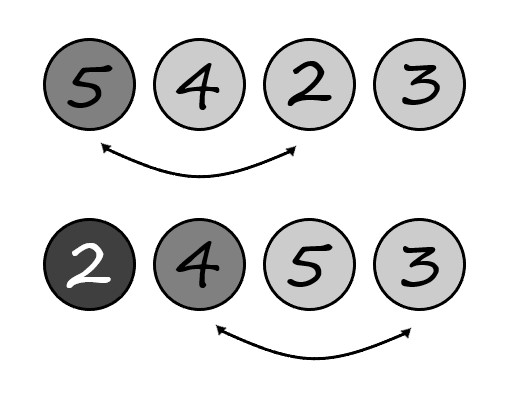
\includegraphics[width=.65\textwidth]{figs/selectionSort.jpg}
  \caption{
    مراحلی از مرتب کردن اعداد به کمک مرتب‌سازی انتخابی
  }
  \label{fig:f2}
\end{figure}

\subsection*{الگوریتم مرتب‌سازی انتخابی}
از اولین عنصر آرایه شروع می‌کنیم. اگر به عنصر
$i$
برسیم،
$i$
را به عنوان اندیسِ\LTRfootnote{index}
کوچک‌ترین عنصر ذخیره می‌کنیم؛
سپس از عنصر بعد از
$i$
شروع می‌کنیم و جلو می‌رویم.
اگر عنصری از
کوچک‌ترین عنصر
کوچک‌تر بود
اندیس آن را به عنوان اندیس کوچک‌ترین عنصر نگه می‌داریم.
وقتی به آخر آرایه رسیدیم،
کوچک‌ترین عنصر ذخیره شده را با
$i$
جابه‌جا\LTRfootnote{swap}
می‌کنیم
و به سراغ عنصر بعدی می‌رویم.
مراحل گفته شده را برای
$i$
جدید تکرار می‌کنیم
تا به انتهای آرایه برسیم.
شبه‌کد مرتب‌سازی انتخابی در
\cref{alg:a2}
که در ادامه آمده است قابل مشاهده است.
همچنین شبه‌کد جابه‌جایی را می‌توانید در
\cref{alg:a3}
مشاهده کنید.

\begin{algorithm}[H]
  \caption{مرتب‌سازی انتخابی}
  \label{alg:a2}
  \begin{latin}
    \begin{algorithmic}[1]
      \Procedure{SelectionSort}{arr, n}
      \For {$i \gets 0$ \textbf{to} $n-1$}
      \State $minIndex \gets i$
      \For {$j \gets i+1$ \textbf{to} $n$}
      \If{$arr[j] < arr[minIndex]$}
      \State $minIndex \gets j$
      \EndIf
      \EndFor
      \State \Call{Swap}{$arr, i, minIndex$}
      \EndFor
      \EndProcedure
    \end{algorithmic}
  \end{latin}
\end{algorithm}

\begin{algorithm}[H]
  \caption{جابه‌جایی}
  \label{alg:a3}
  \begin{latin}
    \begin{algorithmic}[1]
      \Procedure{Swap}{arr, i, j}
      \State $temp \gets arr[i]$
      \State $arr[i] \gets arr[j]$
      \State $arr[j] \gets temp$
      \EndProcedure
    \end{algorithmic}
  \end{latin}
\end{algorithm}

\begin{example}
  \label{ex:e2}
  اگر
  \cref{alg:a2}
  را روی آرایهٔ
  $[5, 4, 2, 3, 7]$
  اجرا کنیم،
  آرایه بدین صورت مرتب می‌شود:
  \begin{align*}
     & [5, 4, 2, 3, 7] \rightarrow [2, 4, 5, 3, 7] \rightarrow
    [2, 3, 5, 4, 7] \rightarrow [2, 3, 4, 5, 7] \rightarrow    \\
     & [2, 3, 4, 5, 7]
  \end{align*}
\end{example}

\begin{example}
  \label{ex:e3}
  اگر
  \cref{alg:a2}
  را روی آرایهٔ
  $[7, 6, 6, 4, 9]$
  اجرا کنیم،
  آرایه بدین صورت مرتب می‌شود:
  \begin{align*}
     & [7, 6, 6, 4, 9] \rightarrow [4, 6, 6, 7, 9] \rightarrow
    [4, 6, 6, 7, 9] \rightarrow [4, 6, 6, 7, 9] \rightarrow    \\
     & [4, 6, 6, 7, 9]
  \end{align*}
\end{example}

\begin{remark}
  توجه کنید در
  \cref{ex:e3}
  با اینکه آرایه بعد از یک جابه‌جایی مرتب می‌شود،
  الگوریتم به کار خود ادامه می‌دهد و به‌ازای تمام عناصر
  $i$
  تا
  $n-1$
  اجرا می‌شود.
  با مقایسه
  \cref{ex:e2}
  و
  \cref{ex:e3}
  که در بالا آمده اند،
  می‌توان وابسته نبودن مرتب‌سازی انتخابی به عناصر ورودی را بهتر درک کرد.
\end{remark}


\section{مرتب‌سازی ادغامی\protect\LTRfootnote{Merge sort}}
مرتب‌سازی ادغامی یکی دیگر از روش‌های مرتب سازی است که از روش تقسیم و حل\LTRfootnote{divide and conquer}
استفاده می‌کند.
این روش در سال ۱۹۴۵ میلادی ابداع شد.
\cite{art}
استفاده از این روش نسبت به روش‌های قبلی سرعت مرتب شدن اعداد را به طور قابل توجهی بالا می‌برد.

این روش اینگونه عمل می‌کند که آرایه را به دو قسمت تقسیم می‌کند و هر قسمت را به صورت بازگشتی مرتب می‌کند.
وقتی که دو قسمت آرایه مرتب شدند، در واقع دو آرایه مرتب شده داریم و می‌خواهیم آن دو را باهم ادغام\LTRfootnote{merge} کنیم.
ادغام کردن دو آرایه مرتب شده و تبدیل آن به یک آرایه مرتب شده، در زمان خطی\LTRfootnote{linear}
قابل انجام است. خطی بودن ادغام یکی از دلایل سریع شدن مرتب‌سازی درجی است.

\subsection*{الگوریتم مرتب‌سازی ادغامی}
آرایه اولیه را به دو قسمت، که اندازه هر قسمت حدود نصف آرایه اولیه است، تقسیم می‌کنیم.
این عمل را به طور بازگشتی ادامه می‌دهیم تا به آرایه‌هایی به یک عضو برسیم.
آرایه با یک عضو همواره مرتب است.
سپس آرایه‌های کوچک‌تر مرتب شده را با یکدیگر ادغام می‌کنیم تا آرایه‌های بزرگتر مرتب شده داشته باشیم.
این عمل را روی کل آرایه انجام می‌دهیم و کل آرایه مرتب می‌شود.
شبه‌کد مرتب‌سازی ادغامی و شبه‌کد ادغام\LTRfootnote{merge}
، که در مرتب‌سازی ادغامی استفاده می‌شود،
به ترتیب در
\cref{alg:a4}
و
\cref{alg:a5}
در ادامه آمده است.
\begin{algorithm}[H]
  \caption{مرتب‌سازی ادغامی}
  \label{alg:a4}
  \begin{latin}
    \begin{algorithmic}[1]
      \Procedure{MergeSort}{$arr, left, right$}
      \If{$left < right$}
      \State $middle \gets \frac{{left + right}}{2}$
      \State \Call{MergeSort}{$arr, left, middle$}
      \State \Call{MergeSort}{$arr, middle + 1, right$}
      \State \Call{Merge}{$arr, left, middle, right$}
      \EndIf
      \EndProcedure
    \end{algorithmic}
  \end{latin}
\end{algorithm}

\begin{algorithm}[H]
  \caption{ادغام}
  \label{alg:a5}
  \begin{latin}
    \begin{algorithmic}[1]
      \Procedure{Merge}{$arr, left, middle, right$}
      \State $n1 \gets middle - left + 1$
      \State $n2 \gets right - middle$

      \State $leftArr \gets \text{new Array}[n1]$
      \State $rightArr \gets \text{new Array}[n2]$

      \For{$i \gets 0$ to $n1$}
      \State $leftArr[i] \gets arr[left + i]$
      \EndFor

      \For{$j \gets 0$ to $n2$}
      \State $rightArr[j] \gets arr[middle + 1 + j]$
      \EndFor

      \State $i \gets 0$
      \State $j \gets 0$
      \State $k \gets left$

      \While{$i < n1$ and $j < n2$}
      \If{$leftArr[i] \leq rightArr[j]$}
      \State $arr[k] \gets leftArr[i]$
      \State $i \gets i + 1$
      \Else
      \State $arr[k] \gets rightArr[j]$
      \State $j \gets j + 1$
      \EndIf
      \State $k \gets k + 1$
      \EndWhile

      \While{$i < n1$}
      \State $arr[k] \gets leftArr[i]$
      \State $i \gets i + 1$
      \State $k \gets k + 1$
      \EndWhile

      \While{$j < n2$}
      \State $arr[k] \gets rightArr[j]$
      \State $j \gets j + 1$
      \State $k \gets k + 1$
      \EndWhile
      \EndProcedure
    \end{algorithmic}
  \end{latin}
\end{algorithm}

\begin{example}
  اگر
  \cref{alg:a4}
  را روی آرایهٔ
  $[7, 6, 3, 1]$
  اجرا کنیم،
  آرایه بدین صورت مرتب می‌شود:
  \begin{align*}
     & [7, 6, 3, 1] \rightarrow [7, 6], [3, 1] \rightarrow
    [7], [6], [3, 1] \rightarrow [6, 7], [3, 1] \rightarrow    \\
     & [6, 7], [3], [1] \rightarrow [6, 7], [1, 3] \rightarrow
    [1, 3, 6, 7]
  \end{align*}
\end{example}

\begin{remark}
  مرتب‌سازی ادغامی نسبت به مرتب‌سازی‌های دیگری که در این مقاله بحث شده
  به حافظه بیشتری نیاز دارد. البته قابل توجه است که اقداماتی برای تغییر این الگوریتم
  با این هدف که پیچیدگی حافظه آن کم شود انجام شده.
  چندین روش برای مرتب‌سازی ادغامی با حافظه ثابت\LTRfootnote{constant}
  یا به عبارتی مرتب سازی ادغامیِ درجا\LTRfootnote{in-place merge sort}
  پیشنهاد شده است.
  \cite{merge1}
\end{remark}

\section{مرتب‌سازی سریع\protect\LTRfootnote{Quicksort}}
مرتب‌سازی سریع یکی از روش‌های پراستفاده برای مرتب‌سازی است.
این روش نه‌تنها سرعت بالایی دارد، بلکه از نظر حافظه نیز خوب عمل می‌کند و حافظه نسبتا کمی استفاده می‌کند.
یکی دیگر از مزایای مرتب سازی سریع این است که الگوریتم نسبتا ساده‌ای دارد
و پیاده سازی آن دشوار نیست.
این الگوریتم توسط تونی هور\LTRfootnote{Tony Hoare}
در سال 1959 میلادی ابداع شد.\cite{quick0}
این روش به طور کلی، در مرتب کردنِ داده‌های تصادفی، از مرتب‌سازی ادغامی
سریع‌تر عمل می‌کند؛ مخصوصا در داده‌های بزرگ‌تر.\cite{quick1}

مرتب‌سازی سریع نیز همانند مرتب‌سازی ادغامی
از روش تقسیم و حل\LTRfootnote{divide and conquer}
استفاده می‌کند.
ابتدا یک عنصر محوری\LTRfootnote{pivot}
انتخاب می‌کند؛ سپس عناصر کوچک‌تر را سمت چپ
و عناصر بزرگ‌تر را در سمت راست آن قرار می‌دهد.
به همین دلیل این روش، مرتب‌سازی بخش‌کردن-تبادل\LTRfootnote{partition-exchange sort}
نیز نامیده می‌شود.\cite{quick2}


\subsection*{الگوریتم مرتب‌سازی سریع}

مرتب سازی سریع به این شکل عمل می‌کند که ابتدا یک عنصر محوری را انتخاب می‌کنیم
.سپس لیست را به دو بخش تقسیم می‌کنیم،
یک بخش برای عناصری که کوچکتر یا مساوی عنصر محوری هستند
و دیگری برای عناصری که بزرگتر از عنصر محوری هستند.
عنصر محوری می‌تواند هر عنصری باشد مثلا برای راحتی می‌توانیم عنصر اول آرایه را در نظر بگیریم.
ولی برای اینکه پیچیدگی زمانی الگوریتم بهینه شود و الگوریتم سریع‌تر عمل کند، این عنصر را با استفاده از
الگوریتم دیگری به نام بخش کردن\LTRfootnote{partition}
انتخاب می‌کنیم.

پس از انتخاب عنصر محوری و تقسیم آرایه به دو بخش، این دو بخش را به طور مستقل مرتب می‌کنیم،
با این معنی که برای هر بخش، عنصر محوری جدیدی را انتخاب می‌کنیم و عملیات تقسیم و حل را بر روی آن اجرا می‌کنیم. این فرایند تا زمانی ادامه می‌یابد که دیگر نتوان بخش‌ها را به زیربخش‌هایی کوچکتر تقسیم کرد.
در انتها، وقتی که همه بخش‌ها به صورت مرتب شده باشند، آنها را با هم ترکیب می‌کنیم
و آرایه به صورت کامل مرتب می‌شود.
شبه‌کد مرتب سازی سریع و بخش کردن را به ترتیب در ادامه در
\cref{alg:a5}
و
\cref{alg:a6}
مشاهده می‌کنید.

\begin{algorithm}[H]
  \caption{مرتب‌سازی سریع}
  \label{alg:a5}
  \begin{latin}
    \begin{algorithmic}[1]
      \Procedure{QuickSort}{$arr, low, high$}
      \If{$low < high$}
      \State $pivot \gets$ \Call{Partition}{$arr, low, high$}
      \State \Call{QuickSort}{$arr, low, pivot - 1$}
      \State \Call{QuickSort}{$arr, pivot + 1, high$}
      \EndIf
      \EndProcedure
    \end{algorithmic}
  \end{latin}
\end{algorithm}

\begin{algorithm}[H]
  \caption{بخش کردن}
  \label{alg:a6}
  \begin{latin}
    \begin{algorithmic}[1]
      \Procedure{Partition}{$arr, low, high$}
      \State $pivot \gets arr[high]$
      \State $i \gets low - 1$
      \For{$j \gets low$ to $high - 1$}
      \If{$arr[j] \leq pivot$}
      \State Swap $arr[i+1]$ and $arr[j]$
      \State $i \gets i + 1$
      \EndIf
      \EndFor
      \State Swap $arr[i+1]$ and $arr[high]$
      \State \textbf{return} $i+1$
      \EndProcedure
    \end{algorithmic}
  \end{latin}
\end{algorithm}

\begin{example}
  فرض کنید می‌خواهیم آرایهٔ $[3, 2, 4, 1]$
  را به کمک مرتب‌سازی سریع مرتب کنیم.
  ابتدا یک عنصر محوری انتخاب می‌کنیم.
  مثلا اولین عنصر که ۳ است.
  عناصر کوچک‌تر یعنی ۲ و ۱ را به سمت چپ و
  عناصر بزرگ‌تر یعنی ۴ را به سمت راست می‌بریم.
  آرایه به شکل
  $[2,1,3,4]$
  درمی‌آید.
  در سمت چپِ ۳،
  $[2, 1]$
  و در سمت راست آن $[4]$
  را داریم.
  $[4]$
  یک عنصر دارد و مرتب شده است.
  برای مرتب کردنِ
  $[2, 1]$
  دوباره مراحل بالا را تکرار می‌کنیم.
  ۲
  را به عنوان عنصر محوری انتخاب می‌کنیم و
  عناصر کوچک تر از آن یعنی ۱ را به سمت چپ آن می‌بریم.
  آرایه مرتب می‌شود و به صورت
  [1, 2]
  درمی‌آید.
  وقتی به آرایه کلی نگاه می‌اندازیم مشاهده می‌کنیم که به صورت
  $[1, 2, 3, 4]$
  است و مرتب شده است.


\end{example}

{
\fontsize{12pt}{10pt}\selectfont
\bibliographystyle{ieeetr-fa}
\bibliography{refs}
\addcontentsline{toc}{section}{مراجع}
}

\end{document}